\documentclass[a4paper]{article}

\usepackage[utf8]{inputenc}
\usepackage[T1]{fontenc}
\usepackage{textcomp}
\usepackage[english]{babel}
\usepackage{amsmath, amssymb}
\usepackage{physics}


% figure support
\usepackage{import}
\usepackage{xifthen}
\pdfminorversion=7
\usepackage{pdfpages}
\usepackage{transparent}
\newcommand{\incfig}[1]{%
	\def\svgwidth{\columnwidth}
	\import{./figures/}{#1.pdf_tex}
}

\pdfsuppresswarningpagegroup=1

\title{CS 213 - Data Structures and Algorithms}
\begin{document}
\maketitle	
\section{Introduction}
Twitter's banner problem - the agenda is to analyze this problem and
work towards a solution. (We were supposed to see a video - I missed it lmao)

CEO of twitter - Parag Agarwal - his student. Well anyway. What's the
problem at hand? People post content on twitter. There's some four people
on the banner page of twitter. Those four people will show up to scrapers etc.

Problem: Place "most popular  posts on the top page dynamically - updated every five-ish minutes or so."

If some folk says something super-interesting that has the potential
to go super-viral, then you want to  shove that on the banner page.

So, consider an array of popularity indices. You as a programmer need
to process this. We will work with toy models only - no full sized
user bases and all.

We want to get the most popular from the list. $\mathcal{O}(n)$ to
get \texttt{max},  then there's going to be a hole to plug. One approach - 
sort the list, pop from the stack. This way no holes to be dealt with.
Problem with sorting (in this particular situation) - if a super-interesting post comes in - we will
not be in a position to dynamically adjust the stack to prioritize it.
Also, sorting is something like $\mathcal{O}(n^2)$ - number of cycles
doubles in order of magnitude.  

\begin{figure}[h]
	\centering
	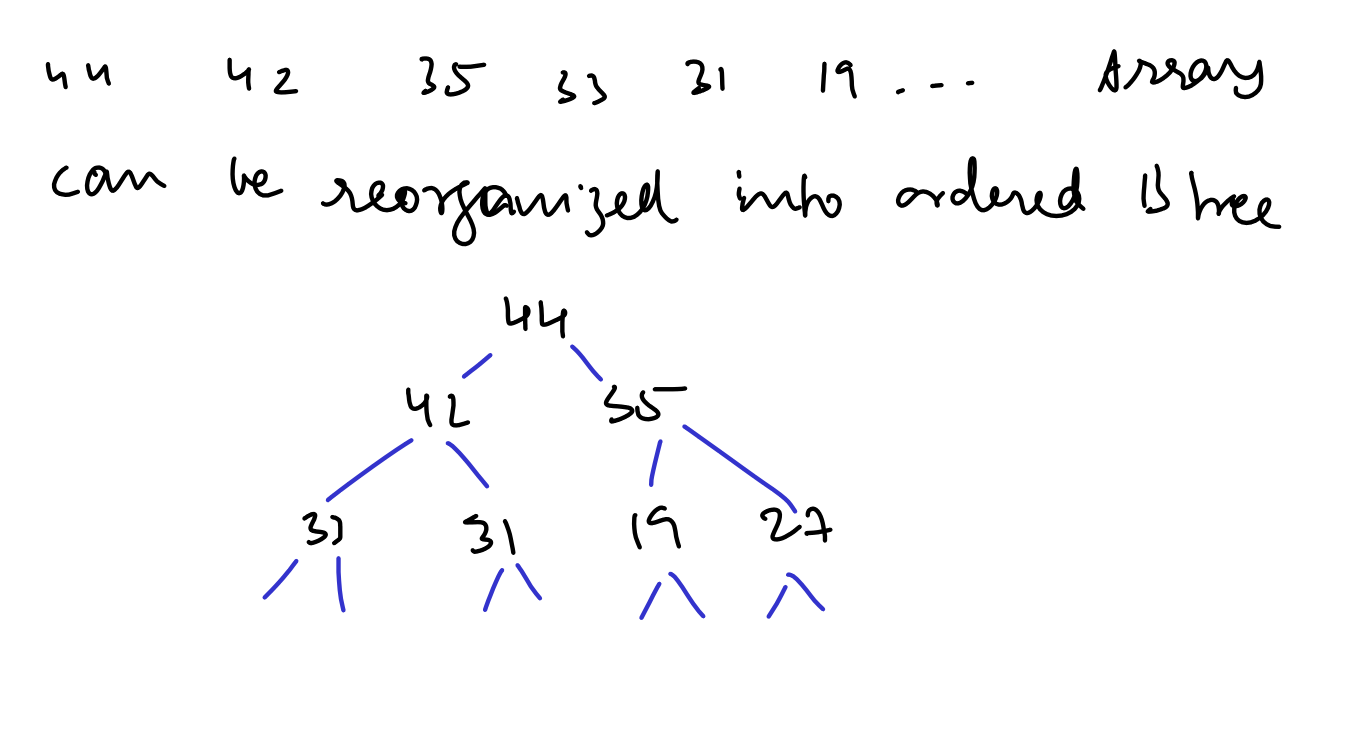
\includegraphics[width=0.8\textwidth]{figures/btree.png}
	\caption{figures/btree.png}
	\label{fig:Ordered binary tree - root, left child, right child}
\end{figure}
The data can be reorganized into another data structure that is more
convenient w.r.t insertions, searching etc. See the above figure.
That is a complete, ordered binary tree (ordered $\implies$ left child
and right child are  distinct for each node, binary $\implies$ two leaves per node, $2^{i}$ nodes in level $i$).

Internally, a binary tree such as this is still stored as an array.
If we want the right child of $j$, we only need realize $j \to 2j+1$.,
which is like ultra easy for the computer.

\begin{itemize}
	\item Right child: $j\to 2j+1$ 
	\item Parent: $k\to \frac{k}{2}$
\end{itemize}
The tree has a 
\begin{itemize}
	\item Structure property: it's a complete B tree
	\item Comparison property: the internal array is sorted - reflects in the B Tree representation
\end{itemize}

So, how would we go about handling the banner problem? The problem
is finding the most popular, next most popular and so on\ldots And
the twist is that there are insertions and deletions happening
dynamically in the internal array. 

So, the first part is \textit{Extract max}.
\begin{figure}[h]
	\centering
	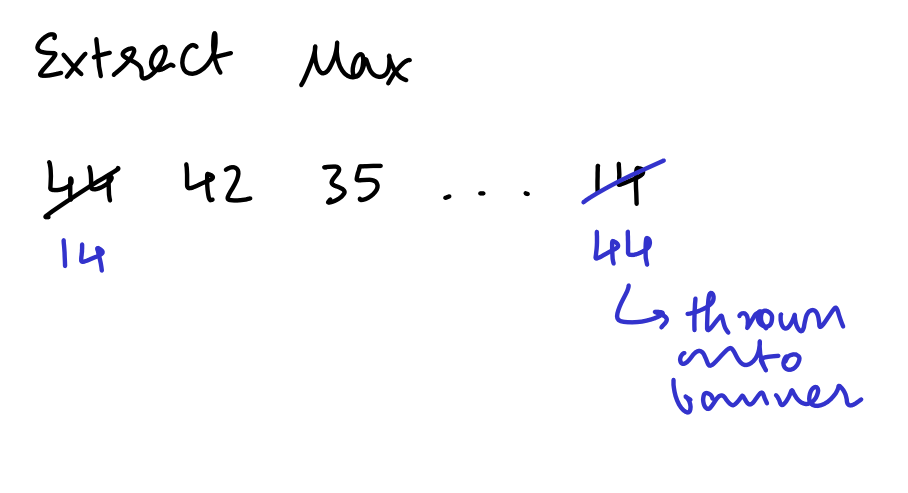
\includegraphics[width=0.8\textwidth]{figures/extractmax.png}
	\caption{figures/extractmax.png}
	\label{fig:Extracting the maximum}
\end{figure}
Consider the figure above. This is what we're doing when we select
the maximum from the array. $44$ and $14$ have been mutually swapped.
But, this destroys the ordering property. 

We can then perform a sequence of operations to fix the order.
\begin{figure}[h]
	\centering
	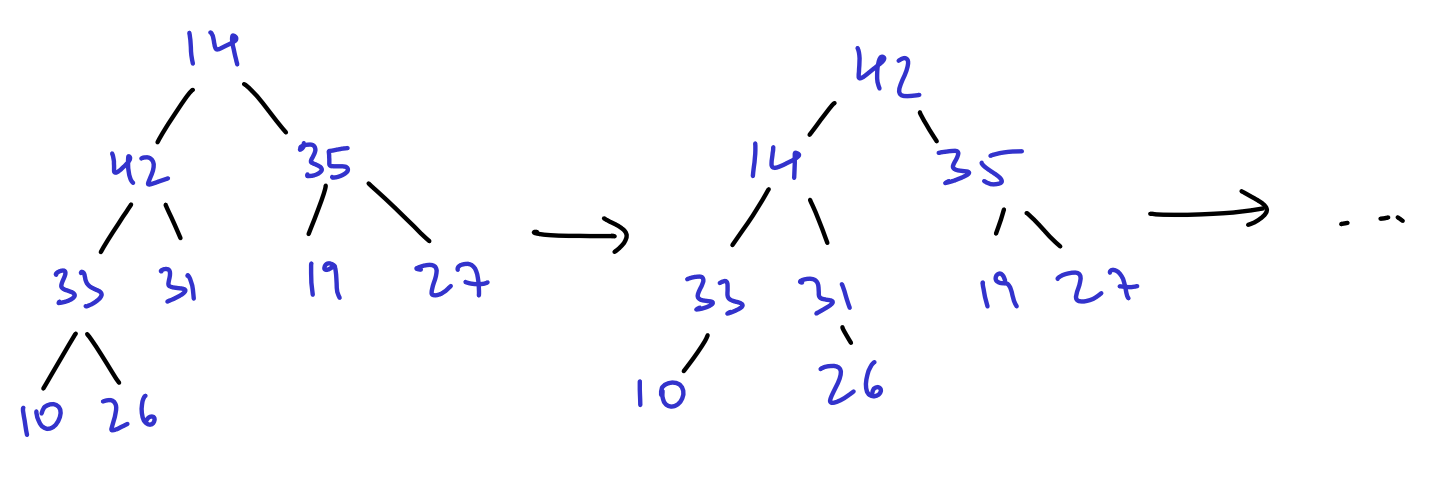
\includegraphics[width=0.8\textwidth]{figures/fix.png}
	\caption{figures/fix.png}
	\label{fig:Fixing the comparison property - propogate down}
\end{figure}
We can keep performing swaps between parent and child as long as we
maintain the invariant that  \texttt{parent} $>$ \texttt{child}.
And because. There will be at most $\log_2n$ comparisons required,
where $n$ is the number of elements in the internal array.

Now, if there is some database trigger and the stack gets updated,
then in general the comparison property will be destroyed. We can
do the same process of sorting them - this time propogating up or
down depending on how the comparisons hold up.

\begin{figure}[h]
	\centering
	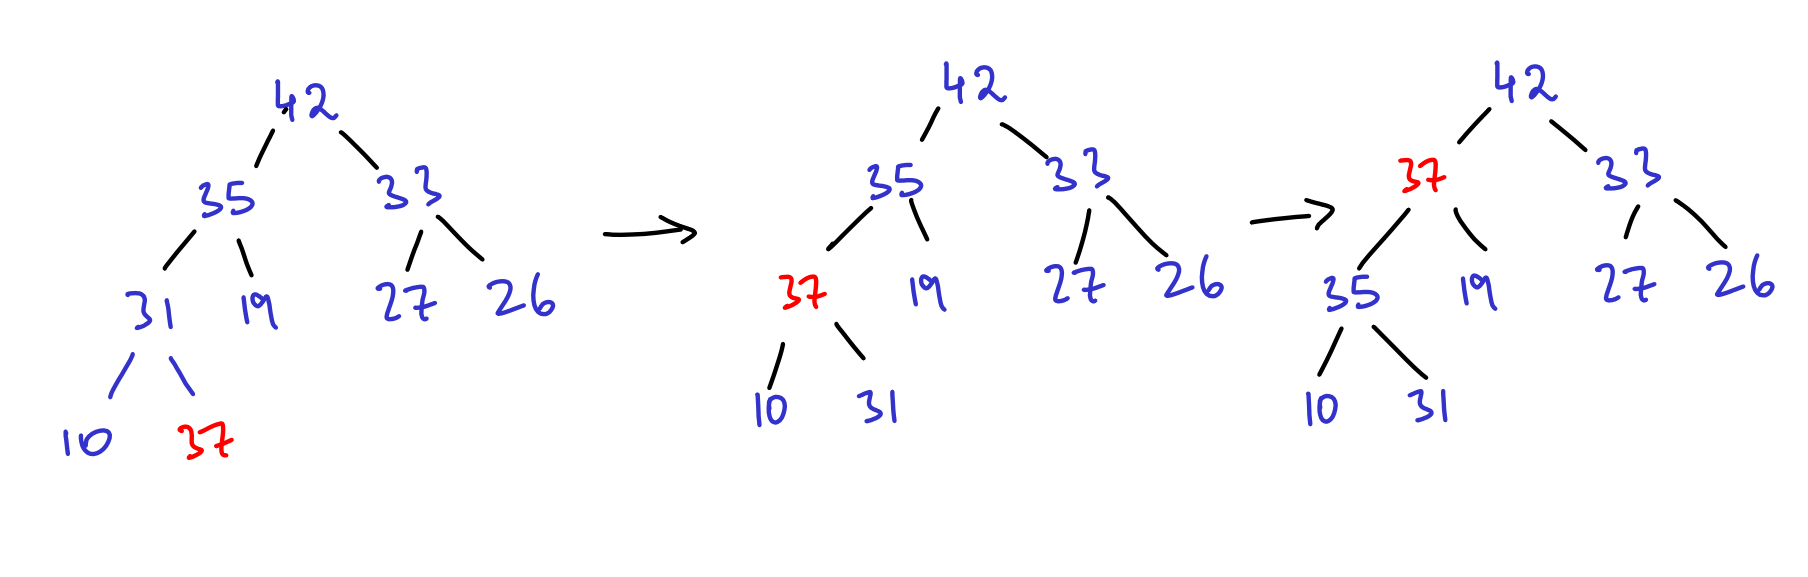
\includegraphics[width=0.8\textwidth]{figures/insertion.png}
	\caption{figures/insertion.png}
	\label{fig: (TODO: verify whether this is right lol) Inserting to heap}
\end{figure}

\textbf{Heap:} a complete binary tree with the comparison property.
Selecting the right data structure is like choosing a scredriver
for a screw that you want to work with. You'd want to choose the best
fit, ya? Don't want to be shoving square cocks in triangle holes.
\end{document}
